\chapter{Uncertainties and sensors calibration}
\label[secinapp]{chap:uncert}
\resetallacronyms

\section{Stable OP}
\label[secinapp]{sec:stable-op}

An \OP{} is considered a stable one if all the sensor values satisfy
one of the following conditions:

\begin{itemize}
\item the value variations are bounded between the following bounds
  for a 3-minute period of time, with at least 100 records.
  \begin{description}
  \item[Temperature] $\pm 0.2$ \si{\degreeCelsius}
  \item[Absolute pressure] $\pm 0.1$ \si{\bar}
  \item[Mass flow rate] $\pm 1$ \%
  \item[Weight] $\pm 1$ \%
  \end{description}
\item The value oscillates steadily around a fixed and stable mean
  value.
\end{itemize}

As stable conditions are set, the measurements are considered as
independent measurements of the same physical value, which greatly
decreases the uncertainty of the measurement, as the uncertainty is
divided by the squared root of the number of measurements $n$, in this
case, as illustrated by \cref{eq:sqrtn}.

\begin{flalign}
  a \pm \dfrac{\Delta a}{\sqrt{n}} \label{eq:sqrtn}
\end{flalign}

\section{Sensors calibration}
\label[secinapp]{sec:calib}

\subsection{Absolute pressure transducers}
\label[secinapp]{sec:bwp-P}

The absolute pressure transducers were calibrated using a dead weight
balance. Some of the pressure transducers have been calibrated
independendly, and some have been calibrated with an other transducer
(two at a time). The dead weight balance used for the calibration is a
device with two chambers: one with oil (oil chamber), which is
pressurized by the application of weights on a vertical piston (weight
support), and one with air (air chamber), where is mounted the
transducer(s) to be calibrated (sensor plug), which is pressurized
using the manual pump and the screw. The goal is to equalize the two
pressures, as the pressure applied by the weights is known. The
transducers signals are recorded at a frequency of 20Hz. The following
procedure is followed to take each of the calibration points.

\paragraph{Procedure:}

The sensor(s) is/are mounted on the dead weight balance. Then the
following protocols are applied:

\subparagraph{At the beginning (no weight on the balance):}

\begin{enumerate}
\item The ball valve is open and the screw is about at the
  middle of its range.
\item The weight support applies a pressure of 0.2 bara on the oil
  chamber. The pressure in the air chamber is increased using
  the pump until the weight support takes off and reaches its
  maximum position.
\item The ball valve is closed and the pressure in the air chamber
  is decreased by rotating the screw until the weight support
  lands again.
\item The air chamber is pressurized again using the screw,
  slowly, until the weight support takes off again by about 5 mm
  (so it does not reach its maximum position). The pressures are now
  equalized.
\item 10 seconds of stable transducer signal is recorded.
\end{enumerate}

\subparagraph{When the weight is increasing:}

\begin{enumerate}
\item The weight is increased by adding a weight on the the weight
  support. The weight support lands because adding
  a weight increases the pressure in the oil chamber. The
  pressures in the two chambers are not egual anymore.
\item The ball valve is open.
\item The air chamber is pressurized using the pump until the
  weight support takes off and reaches its maximum position.
\item The ball valve is closed and the pressure in the air chamber
  is decreased by rotating the screw until the weight support
  lands again. The weights now need to rotate with the weight
  support in order to increase the accuracy of the settings. The
  pressure in the air chamber is increased again using the screw,
  slowly, while the weights rotate, until the weight support takes
  off again. The support rises by about 5 mm and does not reach
  its maximum position. The pressures are now equalized.
\item 10 seconds of stable transducer signal is recorded while the
  weights are rotating.
\end{enumerate}

\subparagraph{When the weight is decreasing:}

\begin{enumerate}
\item The weight is decreased by removing a weight on the the weight
  support. The weight support takes off and reaches
  its maximum position because removing a weight decreases the
  pressure in the oil chamber. The pressures in the two chambers
  are not egual anymore.
\item The weights are rotating.
\item The pressure in the air chamber is decreased using the screw
  until the weight support lands (this operation is done while
  the weights are rotating).
\item The pressure in the air chamber is increased using the screw,
  slowly, until the weight support takes off again (this operation
  is done while the weights are rotating). The support rises by
  about 5 mm and does not reach its maximum position. The pressures
  are now equalized.
\item 10 seconds of stable transducer signal is recorded while the
  weights are rotating.
\end{enumerate}

The pressures were corrected taking into consideration the atmospheric
pressure at the time of the calibration and fitted through a linear
interpolation against the voltage data. For each calibration data
point, the error between the calibration and the measured pressure was
calculated. From that data, the overall uncertainty of the absolute
pressure data was characterized through the mean and standard
deviation of the calibration errors.

\paragraph{Results:}

Calibration statistics for the absolute pressure transducers are
showed on \figref{fig:bwp-P-calib-stats}.

\begin{figure}[h!htbp]
  \centering
  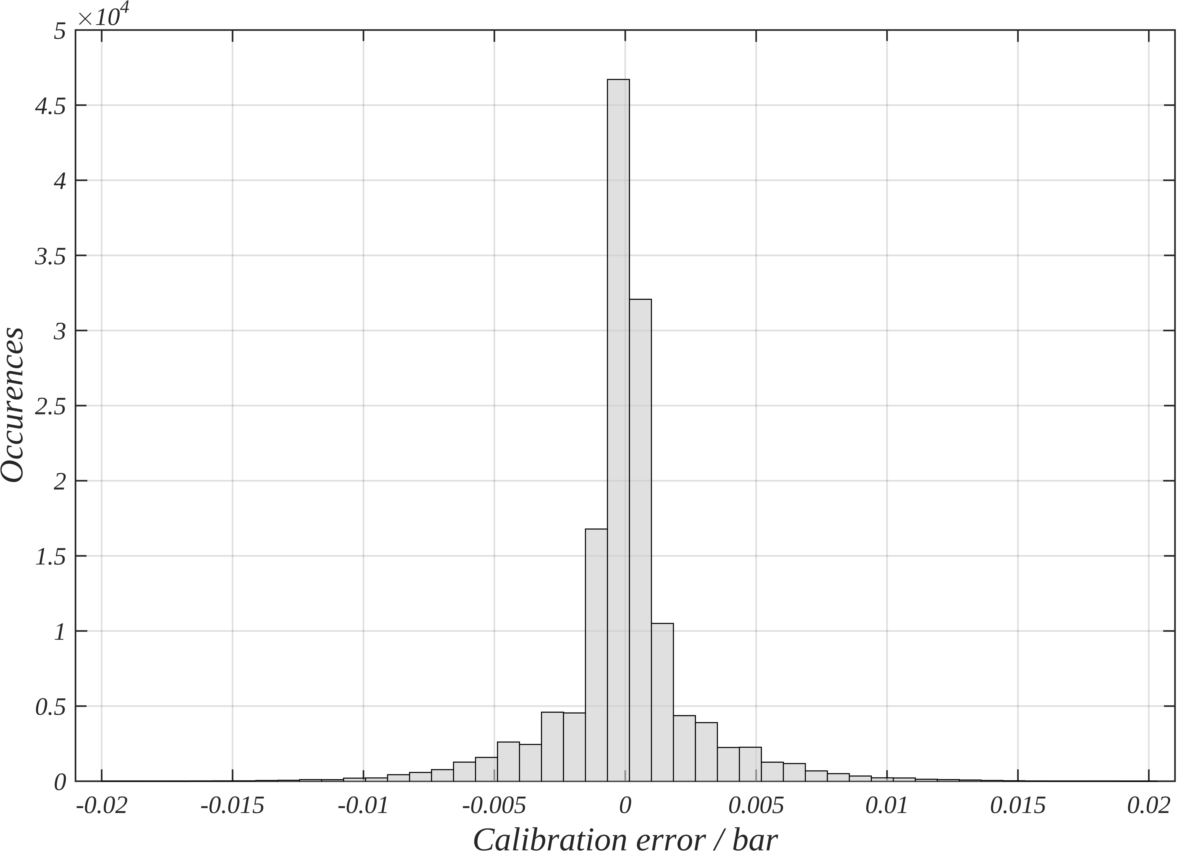
\includegraphics[width=0.45\textwidth]{pressure-calib}
  \caption{Absolute pressure transducers calibration statistics}
  \label{fig:bwp-P-calib-stats}
\end{figure}

\subsection{Thermocouples}
\label[secinapp]{sec:bwp-T}

The temperatures are derived from thermocouple measurements. The
thermocouples used are K-type thermocouples. A thermocouple is a
device made of 2 different conductive materials. In order to measure
the temperature of the medium, the difference of potential created by
the difference of temperature between the two ends of those two
conductive wires is measured and converted into a temperature. The two
ends of the two wires are welded together. In order to be converted
into an absolute temperature, one of the temperatures at the ends of
the wires need to be known. The later can be measured by another
temperature measurement device (usually, a PT100), or kept at a known
value, for example by keeping the wire end into a mixture of ice and
water (the medium is then kept at 0°C)
\citep[p. 5]{rapin-jacquard-2010a}.

\paragraph{Procedure:}

The thermocouples are calibrated against two reference thermometers
PT100 and were calibrated inside a thermally controlled liquid
water-glycol mixture bath. The temperature of the liquid bath has been
varied by steps of 5\si{\degreeCelsius}, first decreasing from 20°C to
-20°C, them incresing from -20°C to 80°C, then decreasing from 80°C to
20°C. Each step has last for 1 hour. The temperatures were stabilizing
after about 30 minutes, them there were 20 minutes of stable signals,
and 10 minutes of recording of stable signals. All the thermocouples
have been calibrated together, at the same time, in the same thermally
controlled bath. The sensors where kept at a homogeneous temperature
being fit into a metallic part drilled to welcome thermocouples. The
part was completely immerged in the thermal bath fluid.

The measured temperatures were fitted through a quadratic
interpolation against the reference data. For each calibration data,
the difference between the calibration and the reference was
calculated. From that data, the overall uncertainty of the temperature
data was characterized through the mean and standard deviation of the
calibrated errors.

\paragraph{Results:}

Calibration statistics for the thermocouples are showed on
\figref{fig:bwp-T-calib-stats}.

\begin{figure}[h!htbp]
  \centering
  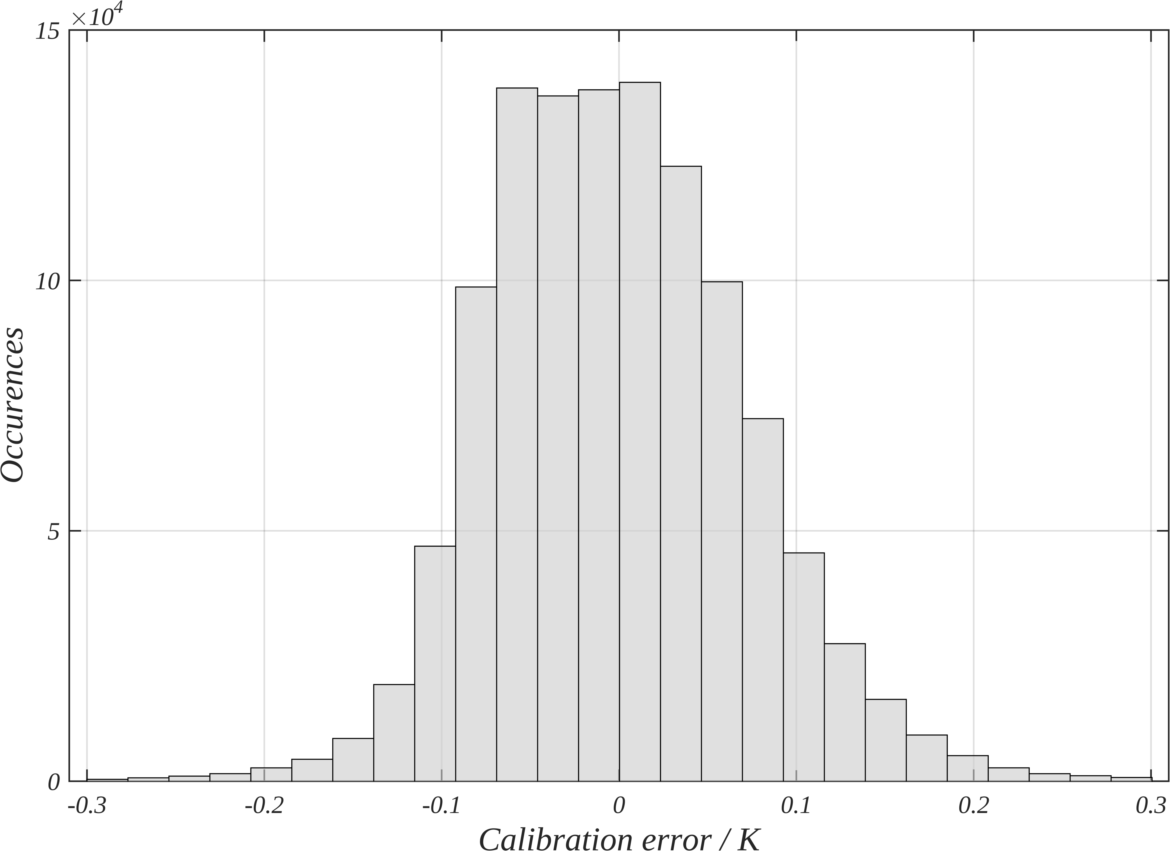
\includegraphics[width=0.45\textwidth]{thermocouple-calib-diff-hist}
  \caption{Thermocouples calibration statistics}
  \label{fig:bwp-T-calib-stats}
\end{figure}

The uncertainty of all the thermocouples is set to the rounded value
of the sum of the mean error, eguals to zero, and twice the standard
deviation, eguals to 0.02\si{\degreeCelsius}. The uncertainty of the
reference probe has been neglected and should have been added. The
uncertainty is rounded above the computed value.

\begin{equation}
  \label{eq:bwp-T-uncert}
  \mu + 2\sigma + \epsilon_{probes} = \pm 0.07\text{°C}
\end{equation}

\section{Uncertainties}
\label[secinapp]{sec:uncert}

\subsection{Propagation of the uncertainties in the calculations}
\label[secinapp]{sec:uncert-propag}

The propagation of the uncertainties through the sets of equations is
performed automatically with the use of class of object in MATLAB,
developed during the thesis \citep{carre-2015a}. The class includes
the following propagation rules.

\subsubsection{Addition \& subtraction}

\begin{flalign}
  & a \pm \Delta a \nonumber \\
  & b \pm \Delta b \nonumber \\
  & (a + b) \pm \sqrt{\Delta a^2 + \Delta b^2}
\end{flalign}

\begin{flalign}
  & a \pm \Delta a \nonumber \\
  & b \pm \Delta b \nonumber \\
  & (a - b) \pm \sqrt{\Delta a^2 + \Delta b^2}
\end{flalign}


\subsubsection{Multiplication \& division}

\begin{flalign}
  & a \pm \Delta a \nonumber \\
  & b \pm \Delta b \nonumber \\
  & a \times b \pm \sqrt{\dfrac{\Delta a}{a}^2 + \dfrac{\Delta b}{b}^2}
\end{flalign}

\begin{flalign}
  & a \pm \Delta a \nonumber \\
  & b \pm \Delta b \nonumber \\
  & \dfrac{a}{b} \pm \sqrt{\dfrac{\Delta a}{a}^2 + \dfrac{\Delta b}{b}^2}
\end{flalign}


\subsubsection{Logarithm \& power}

\begin{flalign}
  & a \pm \Delta a \nonumber \\
  & ln\left(a\right) \pm \sqrt{\dfrac{\Delta a}{a}^2}
\end{flalign}

\begin{flalign}
  & a \pm \Delta a \nonumber \\
  & log\left(a\right) \pm \sqrt{\left(\dfrac{\Delta a}{ln\left(10\right)} \, a \right)^2}
\end{flalign}


\begin{flalign}
  & a \pm \Delta a \nonumber \\
  & b \pm \Delta b \nonumber \\
  & a^b \pm \sqrt{a^b \, \left( b \, \dfrac{\Delta a}{a} \right)^2 + \left( ln(a) \,
    \Delta b \right)^2}
\end{flalign}

\subsubsection{Square root}

\begin{flalign}
  & a \pm \Delta a \nonumber \\
  & \sqrt{a} \pm \sqrt{a \, \left( \dfrac{\Delta a}{2a} \right)^2}
\end{flalign}

\FloatBarrier
\bibliographystyle{plainnat}
\bibliography{main}
\label[secinapp]{sec:uncert-refs}
